% CVPR 2022 Paper Template
% based on the CVPR template provided by Ming-Ming Cheng (https://github.com/MCG-NKU/CVPR_Template)
% modified and extended by Stefan Roth (stefan.roth@NOSPAMtu-darmstadt.de)

\documentclass[10pt,twocolumn,letterpaper]{article}

%%%%%%%%% PAPER TYPE  - PLEASE UPDATE FOR FINAL VERSION
% \usepackage[review]{cvpr}      % To produce the REVIEW version
% \usepackage{cvpr}              % To produce the CAMERA-READY version
\usepackage[pagenumbers]{cvpr} % To force page numbers, e.g. for an arXiv version

% Include other packages here, before hyperref.
\usepackage{graphicx}
\usepackage{amsmath}
\usepackage{amssymb}
\usepackage{booktabs}
\usepackage{lipsum}
\usepackage{tikz}
\usepackage{relsize}
\usepackage{pgfplots}
\usepackage{pgfplotstable}
\usepackage{subcaption}
% \usepackage{float}
\pgfplotsset{compat=1.7}


% It is strongly recommended to use hyperref, especially for the review version.
% hyperref with option pagebackref eases the reviewers' job.
% Please disable hyperref *only* if you encounter grave issues, e.g. with the
% file validation for the camera-ready version.
%
% If you comment hyperref and then uncomment it, you should delete
% ReviewTempalte.aux before re-running LaTeX.
% (Or just hit 'q' on the first LaTeX run, let it finish, and you
%  should be clear).
\usepackage[pagebackref,breaklinks,colorlinks]{hyperref}


% Support for easy cross-referencing
\usepackage[capitalize]{cleveref}
\crefname{section}{Sec.}{Secs.}
\Crefname{section}{Section}{Sections}
\Crefname{table}{Table}{Tables}
\crefname{table}{Tab.}{Tabs.}


%%%%%%%%% PAPER ID  - PLEASE UPDATE
\def\cvprPaperID{*****} % *** Enter the CVPR Paper ID here
\def\confName{CVPR}
\def\confYear{2022}

\newcommand\m[1]{
    \ensuremath{
        \begin{bmatrix}#1\end{bmatrix}
        }
    }

\begin{document}

%%%%%%%%% TITLE - PLEASE UPDATE
\title{Adversarially Robust Medical Classification via Attentive Convolutional Neural Networks}

\author{Isaac Wasserman\\
  University of Pennsylvania\\
  {\tt\small isaacrw@seas.upenn.edu}
}
\maketitle

%%%%%%%%% ABSTRACT
\begin{abstract}
  Convolutional neural network-based medical image classifiers have been shown to be especially susceptible to adversarial examples. Such instabilities are likely to be unacceptable in the future of automated diagnosis. Though statistical adversarial example detection methods have proven to be effective defense mechanisms, additional research is necessary that investigates the fundamental vulnerabilities of deep-learning-based systems and how best to build models that jointly maximize traditional and robust accuracy. This paper presents the inclusion of attention mechanisms in CNN-based medical image classifiers as a reliable and method for increasing robust accuracy without sacrifice. This method is able to increase robust accuracy by up to 16\% in typical adversarial scenarios and up to 2700\% in extreme cases. Additionally, the behavior in attack scenarios of vanilla CNNs and CNNs with attention is compared through the use Grad-CAM activation mapping.
\end{abstract}

%%%%%%%%% BODY TEXT
\section{Introduction}
  Deep neural networks are critical tools in the computing landscape of today, and they have achieved superhuman performance in many incredibly complex tasks such as protein folding \cite{alphafold} and gaming \cite{muzero}. For years, they have been applied to medical diagnostic tasks and have achieved levels of performance on par with highly trained pathologists, radiologists, and other diagnosticians \cite{medical-cnn-survey}. However, these systems are often relegated to lab settings and clinical decision support systems, as their black-box nature does not inspire the confidence necessary for life-critical environments \cite{NIH-AI}\cite{AI-CDSS}.
  
  The decisions of such models are near impossible for the researchers that created them to understand, let alone the proposed clinical end-user \cite{Med-XAI}. Additionally, neural networks are incredibly vulnerable to adversarial examples, instances $x$ whose true label is certifiably $y$, but the mechanics of the estimator (either inherent to the architecture or specific to the weights) result in a confident and incorrect prediction \cite{Intro-Adv}. These examples can be carefully contrived instances $x^\prime = x + p$ which are extremely similar to a natural instance $x$ but are classified differently, $h(x) \not = h(x^\prime)$. However, adversarial examples aren't just the product of bad-actors. Recent research has demonstrated the existence of many naturally occurring instances which reliably behave adversarially when used as input to popular models \cite{Natural-Adv}. Prior to this discovery, researchers and engineers building models for environments where security and bad-actors were not a concern could somewhat understandably deprioritize adversarial robustness, but with the combination of increased reliance on AI-driven systems, everything we've learned about natural adversarial examples, and the proliferation of civilian-targeted cyber-warfare, secure and reliable neural networks are more important than ever.

  If the goal of medical AI is to increase accessibility to high-quality diagnostics and treatments, humans will need to abdicate their roles in some procedural medical processes where AI succeeds such as image classification and segmentation. Unfortunately, these are also the applications where a well-placed orthopedic pin or speck of dust could make all the difference between a properly and improperly diagnosed patient. For medical applications, natural- and robust-accuracy must be optimized simultaneously and with equal priority.

  This paper proposes a simple architectural suggestion for medical image classification models that greatly increases robust-accuracy without sacrificing natural-accuracy, unlike previous techniques \cite{RobustVsAccuracy}. Additionally, this method only increases the parameter count of ResNet-50-based \cite{ResNet} architectures by less than 1.3\%; therefore, training time and data requirements are not significantly affected. Later sections will carefully compare the behavioral differences between baseline and adjusted architectures to investigate the root-cause of this increased performance.

\section{Related Work}
  \subsection{Vulnerability of Medical Image Models}
    Paschali et al. (2018) was among the first to examine the accuracy of popular medical image classification and segmentation models against adversarial images. Their results showed that current adversarial image perturbation methods were able to decrease accuracy on popular medical classification models by up to 25\% and medical segmentation models by up to 41\%. Based on their limited results, they also concluded that dense blocks and skip connections were correlated with more adversarially robust segmentation and that in classification tasks deeper networks tended to be more robust \cite{Paschali}.

    Finlayson et al. (2019) also looked into the susceptibility of medical diagnosis models to adversarial image attacks. Their inquiry found that, although no methods specific to medical images had been developed, attacks methods developed for natural (i.e. non-medical) images were transferable. This work also considered possible motivations for such attacks on these models, contributing the thought that even if clinicians do not soon relinquish their role to neural networks, insurance companies are likely begin outsourcing payment and authorization decisions to AI systems \cite{Finlayson}.

    Ma and Niu et al. (2021) expanded on the works discussed above, reaching the fascinating conclusion that models designed for medical images were, in fact, more vulnerable to adversarial image attacks. Key to this conclusion was their finding that the medical image models they tested had significantly sharper loss landscapes than their natural image counterparts \cite{MaNiu}. This correlation between sharp loss landscapes and more vulnerable models is outlined by Madry et al. (2017), which attributes this sharpness to overparametrization \cite{Madry}. Ma and Niu et al. (2021) echoes this concern of overcomplexity and also suspects that the salience of intricate textures in medical images may also contribute to their compatibility with adversarial attacks. Additionally, they find that while medical image models are easily fooled by adversarial images, adversarially perturbed medical images are more easily detected than their natural image counterparts; they attribute this property to the tendency of popular attacks to place perturbations outside of the image's salient region \cite{MaNiu}.

  \subsection{Finding Adversarially Robust Architectures}
    Training adversarially robust neural networks is an extremely active area of research. Current best-practices involve adversarial training, in which adversarial examples are included in the training set \cite{Madry}. However, this method serves neither to remedy nor understand the underlying vulnerabilities of neural networks and often comes at the cost of training time and clean accuracy (i.e. accuracy on non-adversarial inputs) \cite{RobustVsAccuracy}. For this reason, it is imperative that the research community continues to investigate architectural modifications that yield greater adversarial robustness.

    In an extensive grid search of CNN architectures for predicting CIFAR-10, Huang et al. (2021) found that while the total number of parameters does not seem to be correlated to robustness, reductions in the depth or width of deeper layers does seem to produce more robust models. However, this relationship was not consistent, and the authors were unable to articulate why it appeared \cite{Huang}.

    Dong et al. (2020) developed an NAS (neural architecture search) algorithm called "Adversarially Robust Neural Architecture Search with Confidence Learning" (RACL) which was shown to produce models that significantly outperformed state-of-the-art models and models produced by other NAS algorithms in terms of both clean- and robust-accuracy. Key to the algorithm's success is its method of approximating and minimizing the lipschitz constant of the resultant model. When combined with adversarial training, RACL scored between 0.43\% and 3.17\% higher than the next best model and had the second-best clean-accuracy of all those tested. Without adversarial training, RACL had the highest clean-accuracy and the highest accuracies against MIM and PGD attacks by 10.64\% and 359.52\% respectively; however, a standard DenseNet-121 outperformed it against FGSM attacks by 21.77\% \cite{RACL}.

    Mok et al. (2021) furthered this work to develop an NAS for finding robust architectures. Called AdvRush, their algorithm prioritizes the smoothness of input loss landscape and uses a novel technique to simultaneously evaluate the robustness of all candidate architectures against perturbations in a two-dimensional projection of the feature-space. In practice the resultant model outperformed state-of-the-art architectures and other NAS algorithms (including RACL) on CIFAR-10 under FGSM, PGD, APGD, and AutoAttack by at least 2.79\%, 3.25\%, 2.82\%, and 3.07\% respectively; and it additionally outperformed all other models in clean-accuracy by at least 1.57\%. However, the model was significantly more complex than those generated by DARTS and RACL, utilizing 17\% more parameters \cite{AdvRush}.

    Despite the multitude of NAS algorithms developed recently \cite{RACL}\cite{AdvRush}\cite{MORAS}\cite{DSRNA}, previous research has not discovered reliable methods or guidelines for building robust architectures. Instead, these algorithms are merely able to efficiently search a finite set of architectures for the most robust option in a given task.

  \subsection{Vision Transformers}
    Recent advances in natural language processing have offered the computer vision research community a new option for image classification, the vision transformer (ViT) \cite{VisionTransformerSurvey}. Models utilizing this family of architectures commonly match or exceed the performance of convolutional neural networks \cite{ViT}\cite{DeiT}\cite{PVT}\cite{Swin}.
    
    Shao et al. (2021) found these architectures to be more adversarially robust than their CNN counterparts. When compared to various versions of ResNet, ShuffleNet, MobileNet, and VGG16, ViT-S/16 was up to 46\% more robust to PGD attacks and 44\% more robust to AutoAttack \cite{RobustTransformers}. In fact, for attack radii less than 0.01, the most robust CNN was less robust than the least robust vision transformer. All the while, the clean accuracy of the transformers was, on average, 7\% higher than that of the CNNs. Additionally, ViT-S/16 (the most robust overall) has just 22 million trainable parameters, compared to the 25 million parameters of ResNet-50 \cite{ViT}\cite{ResNet}.

    Based on their analysis, Shao et al. (2021) found that ViTs tend to learn more robust, high-level features, allowing them to ignore the high frequency perturbations of many attack methods. They also found that in architectures that combined transformer and convolutional blocks, a high proportion of transformer blocks correlated to higher robust-accuracy \cite{RobustTransformers}.

  \subsection{CNNs with Attention}
    \subsubsection{Adversarial Robustness}
      Since their inception, it has been understood that the superior clean-accuracy of vision transformers is related to their reliance on attention \cite{VisionTransformerSurvey}, and recently it has been confirmed that this property is also responsible for the architecture's superior robustness \cite{UnderstandingTransformerRobustness}. Zhou et al. (2022) found that the self-attention of vision transformers tends to promote the saliency of more meaningful (non-spurious) clusters of image regions.

      Working from this knowledge, it is natural to wonder whether attention mechanisms can offer additional adversarial robustness to CNNs. Agrawal et al. (2022) concluded that this was not necessarily the case, finding that while their attentive CNNs had slightly superior robustness to PGD attacks on the CIFAR-100 dataset, it fell behind ResNet-50 on CIFAR-10 and Fashion MNIST. Based on these results, they suspected that the adversarial robustness of attentive models on a given dataset may correlate to the number of classes \cite{AttentiveCNNRobustness}.
    
    \subsubsection{Clean Accuracy}
      Agrawal et al. (2022) also found that the attentive model had slightly lower clean-accuracy compared to the vanilla CNNs on CIFAR-10 and CIFAR-100 but slightly higher clean-accuracy on Fashion MNIST \cite{AttentiveCNNRobustness}. However, this finding is inconsistent with early research on the use of CNNs with attention for fine-grained classification datasets. For example, the attention-based model developed by Xiao et al. (2015) outperformed equally supervised vanilla-CNNs by 19\% \cite{AttentionForFineGrainedClassification}. As small details are incredibly salient in medical image datasets, research on fine-grained classification is especially relevant. The ability of attention mechanisms to improve the accuracy of medical image classification CNNs was confirmed by Datta et al. (2021) which appended a minimal soft-attention mechanism to five off-the-shelf pretrained CNNs and found that attention increased weighted average AUC for all but VGG16 \cite{AttentionSkinCancerClassification}.

      Based on the findings above, it appears possible that the use of attention is a minimal architectural feature that challenges the findings of Tsipras et al. (2018) \cite{RobustVsAccuracy} by improving clean- and robust-accuracy simultaneously.

  \section{Method}
    \subsection{Datasets}
      Benchmark medical image classification tasks were chosen based on their frequent use in similar studies, such as Ma and Niu et al. (2021) \cite{MaNiu} and Finlayson et al. (2019) \cite{Finlayson}. These tasks are diabetic retinopathy detection from fundoscopy images, pneumothorax detection from chest x-rays, and skin lesion classification from dermatoscopy images. Fundoscopy images were sourced from the popular Kaggle diabetic retinopathy detection competition \cite{KaggleDR}. Chest x-rays used were from the ChestX-Ray14 dataset \cite{ChestX-Ray14}. Unlike Finlayson et al. (2019) \cite{Finlayson} and Ma and Niu et al. \cite{MaNiu} (2021), dermatoscopy images were not sourced directly from ISIC \cite{ISIC} and were instead taken from the HAM10000 dataset \cite{HAM10000} which draws from the ISIC archive; this choice was made to more closely resemble the setup of Datta et al. (2021) \cite{AttentionSkinCancerClassification}.

    \subsection{Preprocessing}
      All images were resized to the ImageNet standard $224 \times 224$ pixels \cite{ImageNet} and preprocessed according to the specifications of the TensorFlow \cite{TensorFlow} implementation of ResNet-50 \cite{ResNet}, which include subtracting 123.68, 116.779, and 103.939 from the red, green, and blue channels respectively \cite{ResNetPreprocessingImplementation}.

      The fundoscopy and chest x-ray datasets were distilled from their original multiclass classification form into binary classification datasets. For the fundoscopy images, the "No DR" and "Mild DR" classes were considered negative while the "Moderate," "Severe," and "Proliferative DR" classes were considered positive. The chest x-ray dataset originally included 14 non-exclusive classes, but for the purposes of this study, all images labeled as having a pneumothorax present were labeled positive, while other images were simply labeled negative. No changes were made to the classes of the dermatoscopy dataset.

      In an attempt to solve for the relatively large range in image contrast of the grayscale chest x-rays, all images were put through a gaussian filtering pipeline that maximized the prominence of edges and shadowed areas. Images are first min-max normalized to the range $[0,255]$. A gaussian blur is applied to a copy of this image; the kernel size of the filter is computed based on parameters $\sigma_x=20,\,\,\, \sigma_y=0$. This blurred image $\text{blur}(x)$ is subsequently added to the original normalized image $x$ according to the following formula $x' = 4x - 4(\text{blur}(x)) + 128$.

      \begin{figure}[h!]
        \centering
        $
        \begin{array}{l}
        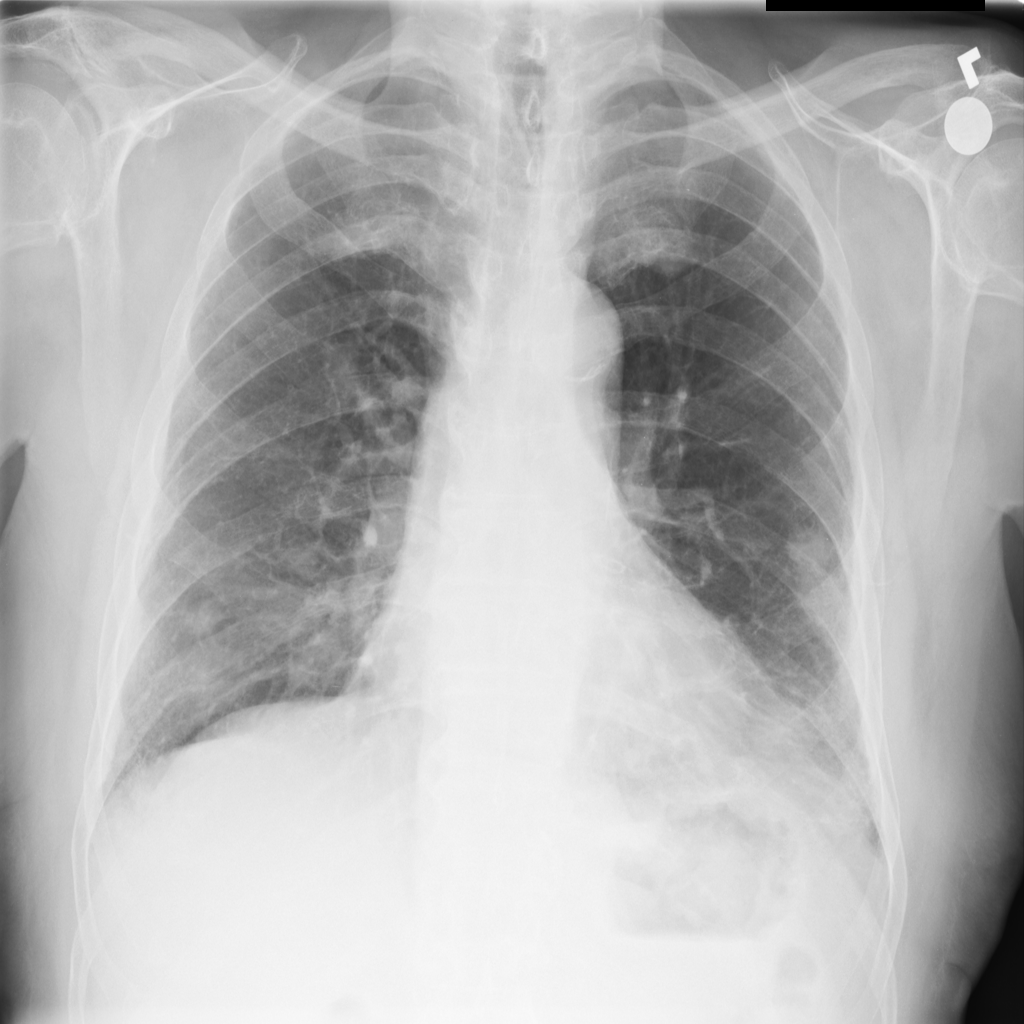
\includegraphics[width=0.4\linewidth]{graphics/ResNet-50/unprocessedxray.png}
        \end{array}
        \mathlarger{\mathlarger{\mathlarger{\mathlarger{\rightarrow}}}}
        \begin{array}{l}
          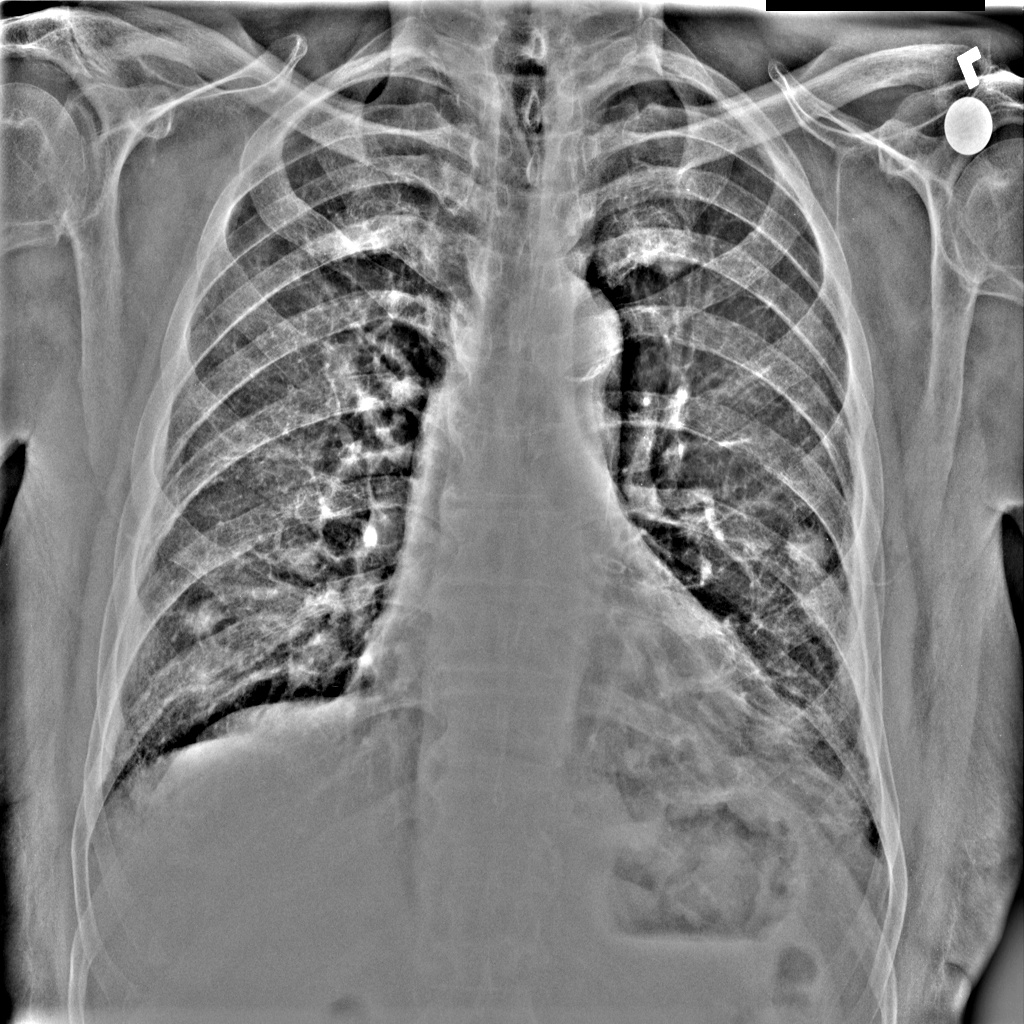
\includegraphics[width=0.4\linewidth]{graphics/ResNet-50/processedxray.jpg}
        \end{array}
        $
        \caption{Visualization of the chest x-ray image preprocessing pipeline}
      \end{figure}

      This pipeline was initially used for the fundoscopy images as well, but early results revealed that this type of processing was not well suited to the task.

    \subsection{Network Architecture}
      Four models were trained for each dataset, a ResNet-50 with and without a soft attention block and an InceptionResNetV2 with and without soft attention. The architecture of each model was based on the TensorFlow \cite{TensorFlow} implementations of ResNet-50 \cite{ResNetImplementation} and InceptionResNetV2 \cite{InceptionImplementation}.
      
      ResNet-50 was instantiated with the top block included, initial weights based on ImageNet \cite{ImageNet} pretraining, and class count set to 1000. The final three layers of the network were removed. In the models without attention, these final layers were replaced with a 2D global average pooling layer followed by a fully-connected layer with softmax activation. In the models with attention, the last three layers were replaced with a soft attention block implemented according to the specifications of Datta et al. (2021). This block produces a $7 \times 7$ feature map which is $2 \times 2$ max pooled and concatenated with a $2 \times 2$ max pooled version of the input to the attention block. This concatenated output is put through ReLU activation, 50\% dropout, and global average pooling before being handed off to the fully connected prediction head with softmax activation \cite{AttentionSkinCancerClassification}.
      
      InceptionResNetV2 \cite{InceptionResNet} was instantiated with the top block included, initial weights based on ImageNet, and classifier activation as softmax. In the models without attention, the final 28 layers were replaced with a ReLU activation and 50\% dropout whose output was flattened and sent to the fully connected prediction head with softmax activation. In the models with attention, these layers were replaced by the soft attention block described above. This output is $2 \times 2$ max pooled and concatenated with a max pooled version of the input to the attention block before being sent through ReLU activation and the softmax prediction head.

      In each model, the width of the prediction head was equal to the number of classes in the dataset (seven for dermatoscopy and two for fundoscopy and chest x-ray).

      All models used the Adam optimizer with $\eta=0.01$ and $\epsilon=0.1$ and minimized categorical cross-entropy during training. During training classes were weighted based on their inverse frequency relative to the other classes. Each model was trained for a maximum of 300 epochs with early stopping (patience $=$ 40, minimum delta $=$ 0.001) causing most to stop after 60-90 epochs. In the dermatoscopy task, models only saw 10\% of the dataset during each epoch; this was done to increase the odds of reproducing the results of Datta et al. (2021) \cite{AttentionSkinCancerClassification}.

    \subsection{Evaluation and Analysis of Robustness}
      After training, the models' clean- and robust-accuracy was evaluated using the FoolBox \cite{FoolBoxPaper}\cite{FoolBoxLibrary} library's implementation of $l_\infty$ projected gradient descent attacks. Each set of models was tested at increasing epsilons (perturbation radii). Attacks of these perturbation radii were created for each image in the test sets. Unweighted accuracy was calculated for each perturbation radius.

      Small samples of the resultant adversarial images were saved and used to analyze model behavior using gradient weighted class activation mapping (Grad-CAM) \cite{Grad-CAM} localization maps. These maps were generated using the Grad-CAM implementation of Datta et al. (2021) \cite{AttentionSkinCancerClassification} and provide attention-map-esque representations of spatial importance for neural networks regardless of whether they utilize attention mechanisms or not. For each model, these maps were generated at each epsilon for 16 sample images with and without perturbations applied. Maps for a given starting image were compared to their perturbed counterpart as well as against other models and perturbation radii.

  \section{Results}
    \subsection{ResNet-50 Models}
      For the task of skin lesion classification, the models with attention are clearly superior, in terms of robustness (Fig. \ref{DermResNet50Robustness}). Although the model without attention has slightly higher clean-accuracy (0.905 vs. 0.88), even the slightest perturbation ($\epsilon=0.00125$) is able to reduce its accuracy by 24\% and put the model with attention in the lead. By the time $\epsilon=0.005$, the model is worse than random, and by the time $\epsilon=0.01$, the model is rendered completely useless. It is worth noting that perturbation of this size (Fig. \ref{example_derm_perturbation}) is far from being human perceptible. Meanwhile, at this perturbation radius, the model with attention remains better than random selection.

      \begin{figure}[h!]
        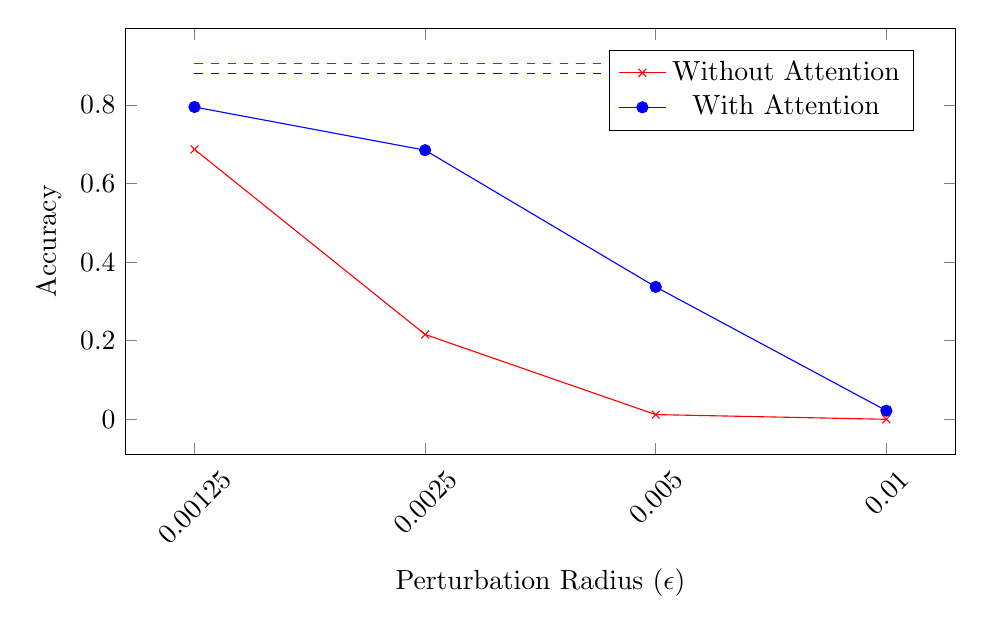
\begin{tikzpicture}
          \begin{axis}[xtick={0, 0.00125, 0.0025, 0.005, 0.01, 0.02, 0.04, 0.08, 0.16, 0.32}, x tick label style={rotate=45, log ticks with fixed point},xmode=log, log basis x=2, xlabel=Perturbation Radius ($\epsilon$), ylabel=Accuracy, width=\linewidth, height=7cm,legend style={at={(0.95,0.95)},anchor=north east}]
              
          \addplot[color=red,mark=x] coordinates {
            (0.00125, 0.687)
            (0.0025, 0.216)
            (0.005, 0.012)
            (0.01, 0)
          };
          
          \addplot[color=blue,mark=*] coordinates {
            (0.00125, 0.795)
            (0.0025, 0.685)
            (0.005, 0.337)
            (0.01, 0.022)
          };

          \addplot[color=red, domain=0.00125:0.01, dashed]{0.905};
          \addplot[color=blue, domain=0.00125:0.01, dashed]{0.880};
          
          \legend{Without Attention,With Attention}
          \end{axis}
          \end{tikzpicture}
        \caption{Clean- and robust-accuracy of ResNet-50 models for skin lesion classification.  Dashed lines represent clean-accuracy.}
        \label{DermResNet50Robustness}
      \end{figure}

      The models for diabetic retinopathy detection tell a slightly different story (Fig. \ref{DRResNet50Robustness}). These models were, overall, much more robust, requiring a perturbation of at least $\epsilon=0.01$ to reduce accuracy by 3\%. As in the skin lesion classification models, the model without attention has a slightly higher clean accuracy (0.832 vs. 0.818). It retains this very small lead until $\epsilon=0.02$, at which point, the accuracy of both models begins falling, but the model with attention does so a bit less dramatically. At the maximum perturbation radius tested ($\epsilon=0.32$) (Fig. \ref{example_dr_perturbation}), the accuracy of the model with attention is over 20 times higher than that of the model without.

      \begin{figure}[h!]
        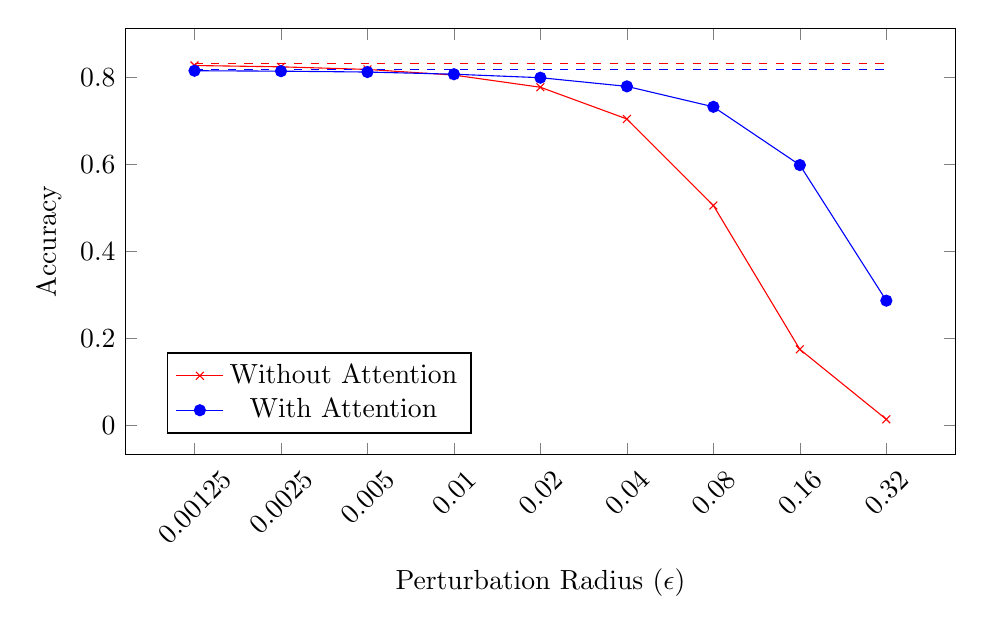
\begin{tikzpicture}
          \begin{axis}[xtick={0, 0.00125, 0.0025, 0.005, 0.01, 0.02, 0.04, 0.08, 0.16, 0.32}, x tick label style={rotate=45, log ticks with fixed point},xmode=log, log basis x=2, xlabel=Perturbation Radius ($\epsilon$), ylabel=Accuracy, width=\linewidth, height=7cm,legend style={at={(0.05,0.05)},anchor=south west}]
              
          \addplot[color=red,mark=x] coordinates {
            (0, 0.832)
            (0.00125, 0.828)
            (0.0025, 0.825)
            (0.005, 0.819)
            (0.01, 0.806)
            (0.02, 0.778)
            (0.04, 0.705)
            (0.08, 0.506)
            (0.16, 0.175)
            (0.32, 0.014)
          };
          
          \addplot[color=blue,mark=*] coordinates {
            (0, 0.818)
            (0.00125, 0.816)
            (0.0025, 0.815)
            (0.005, 0.813)
            (0.01, 0.808)
            (0.02, 0.8)
            (0.04, 0.780)
            (0.08, 0.733)
            (0.16, 0.599)
            (0.32, 0.287)
          };

          \addplot[color=red, domain=0.00125:0.32, dashed]{0.832};
          \addplot[color=blue, domain=0.00125:0.32, dashed]{0.818};
          
          \legend{Without Attention,With Attention}
          \end{axis}
          \end{tikzpicture}
        \caption{Clean- and robust-accuracy of ResNet-50 models for diabetic retinopathy detection. Dashed lines represent clean-accuracy.}
        \label{DRResNet50Robustness}
      \end{figure}

      The pneumothorax detection models, collectively, were even more robust than the diabetic retinopathy detection models (Fig. \ref{PneumoResNet50Robustness}). After perturbations of $\epsilon=0.32$ (Fig. \ref{example_pneumo_perturbation}), the accuracy of both models met at 0.805. Prior to this, the accuracy of the model without attention hovered 1-2\% above that of the model with attention. However, based on the trajectory of the models' accuracy with respect to $\epsilon$, perturbation radii higher than 0.32 would likely result in the model with attention leapfrogging the model without.

      \begin{figure}[h!]
        \begin{subfigure}{\linewidth}
          \centering
          $
          \begin{array}{l}
          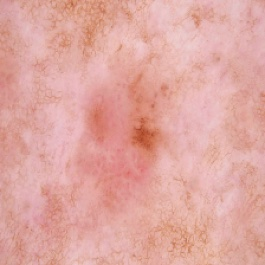
\includegraphics[width=0.26\linewidth]{graphics/ResNet-50/derm_unperturbed.jpg}
          \end{array}
          \mathlarger{\mathlarger{\mathlarger{\mathlarger{+}}}}
          \begin{array}{l}
            
\includegraphics[width=0.26\linewidth]{graphics/ResNet-50/derm_e=0.01_difference.jpg}
          \end{array}
          \mathlarger{\mathlarger{\mathlarger{\mathlarger{=}}}}
          \begin{array}{l}
            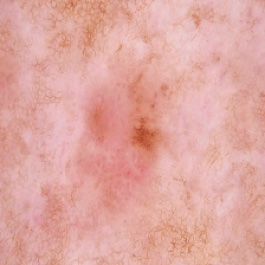
\includegraphics[width=0.26\linewidth]{graphics/ResNet-50/derm_e=0.01.jpg}
          \end{array}
          $
          \caption{An example of $\epsilon=0.01$ perturbation on the dermatoscopy dataset. 0.01 is the maximum perturbation radius used for this dataset.\\}
          \label{example_derm_perturbation}
        \end{subfigure}
        
        \begin{subfigure}{\linewidth}
          \centering
          $
          \begin{array}{l}
          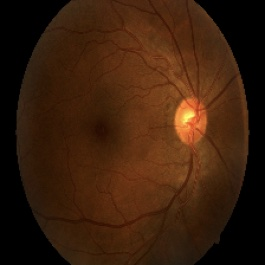
\includegraphics[width=0.26\linewidth]{graphics/ResNet-50/dr_unperturbed.jpg}
          \end{array}
          \mathlarger{\mathlarger{\mathlarger{\mathlarger{+}}}}
          \begin{array}{l}
            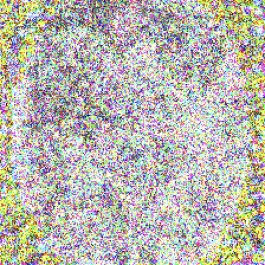
\includegraphics[width=0.26\linewidth]{graphics/ResNet-50/dr_e=0.32_difference.jpg}
          \end{array}
          \mathlarger{\mathlarger{\mathlarger{\mathlarger{=}}}}
          \begin{array}{l}
            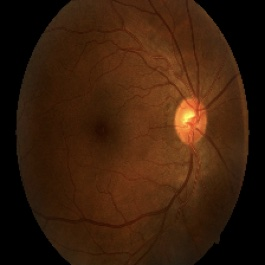
\includegraphics[width=0.26\linewidth]{graphics/ResNet-50/dr_e=0.32.jpg}
          \end{array}
          $
          \caption{An example of $\epsilon=0.32$ perturbation on the fundoscopy dataset. 0.32 is the maximum perturbation radius used for this dataset.\\}
          \label{example_dr_perturbation}
        \end{subfigure}
        \begin{subfigure}{\linewidth}
          \centering
          $
          \begin{array}{l}
          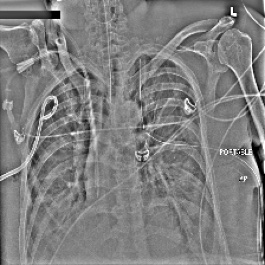
\includegraphics[width=0.26\linewidth]{graphics/ResNet-50/pneumo_unperturbed.jpg}
          \end{array}
          \mathlarger{\mathlarger{\mathlarger{\mathlarger{+}}}}
          \begin{array}{l}
            
\includegraphics[width=0.26\linewidth]{graphics/ResNet-50/pneumo_e=0.32_difference.jpg}
          \end{array}
          \mathlarger{\mathlarger{\mathlarger{\mathlarger{=}}}}
          \begin{array}{l}
            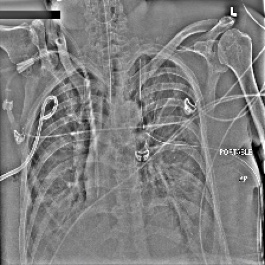
\includegraphics[width=0.26\linewidth]{graphics/ResNet-50/pneumo_e=0.32.jpg}
          \end{array}
          $
          \caption{An example of $\epsilon=0.32$ perturbation on the chest x-ray dataset. 0.32 is the maximum perturbation radius used for this dataset.\\}
          \label{example_pneumo_perturbation}
        \end{subfigure}%
        \caption{Perturbation examples}
      \end{figure}

      \begin{figure}[h!]
        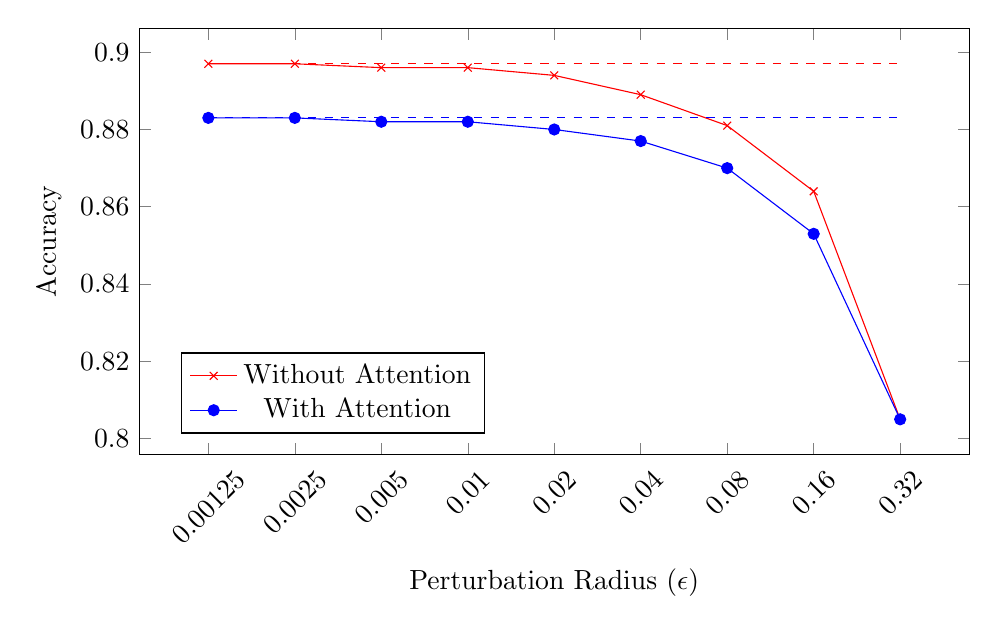
\begin{tikzpicture}
          \begin{axis}[xtick={0, 0.00125, 0.0025, 0.005, 0.01, 0.02, 0.04, 0.08, 0.16, 0.32}, x tick label style={rotate=45, log ticks with fixed point},xmode=log, log basis x=2, xlabel=Perturbation Radius ($\epsilon$), ylabel=Accuracy, width=\linewidth, height=7cm,legend style={at={(0.05,0.05)},anchor=south west}]
              
          \addplot[color=red,mark=x] coordinates {
            (0.00125, 0.897)
            (0.0025, 0.897)
            (0.005, 0.896)
            (0.01, 0.896)
            (0.02, 0.894)
            (0.04, 0.889)
            (0.08, 0.881)
            (0.16, 0.864)
            (0.32, 0.805)
          };
          
          \addplot[color=blue,mark=*] coordinates {
            (0.00125, 0.883)
            (0.0025, 0.883)
            (0.005, 0.882)
            (0.01, 0.882)
            (0.02, 0.880)
            (0.04, 0.877)
            (0.08, 0.870)
            (0.16, 0.853)
            (0.32, 0.805)
          };

          \addplot[color=red, domain=0.00125:0.32, dashed]{0.897};
          \addplot[color=blue, domain=0.00125:0.32, dashed]{0.883};
          
          \legend{Without Attention,With Attention}
          \end{axis}
          \end{tikzpicture}
        \caption{Clean- and robust-accuracy of ResNet-50 models for pneumothorax detection. Dashed lines represent clean-accuracy.}
        \label{PneumoResNet50Robustness}
      \end{figure}

    \subsection{InceptionResNetV2 Models}
  \section{Discussion}
    \subsection{Analysis of Perturbations and Activation Maps}
      In an attempt to better understand the principles and behaviors that led the CNNs with attention to perform better in both clean and adversarial scenarios, perturbation difference maps and Grad-CAM activation maps were generated for a select sample of images on each model. Individually, these difference maps and activation maps were unremarkable. However, a number of dataset specific patterns were noticed throughout the images used for this analysis.
      \subsubsection{ResNet-50 Models}
        While imperceptible in the final images, the perturbations for dermatoscopic and fundoscopic images were found to carry easily perceptible information about the source image, when the changes were scaled to a range of $[0,255]$. In these cases, the adversarial ``noise'' contained the shape of the lesion or eye. For dermatoscopic images, this shape was in the form of a densely perturbed ring enclosing a sparsely perturbed center (Fig. \ref{LesionShape}). This phenomenon was most visible when $\epsilon=0.00125$. For the fundoscopic images, this shape was represented by a sparsely perturbed ellipse. In the attacks generated for the model with attention, the shape of this ellipse occasionally diverged from the true shape of the eye (Fig. \ref{EyeShapeDivergence}).

        \begin{figure}[h]
          \centering
          \begin{subfigure}{.4\linewidth}
            \centering
            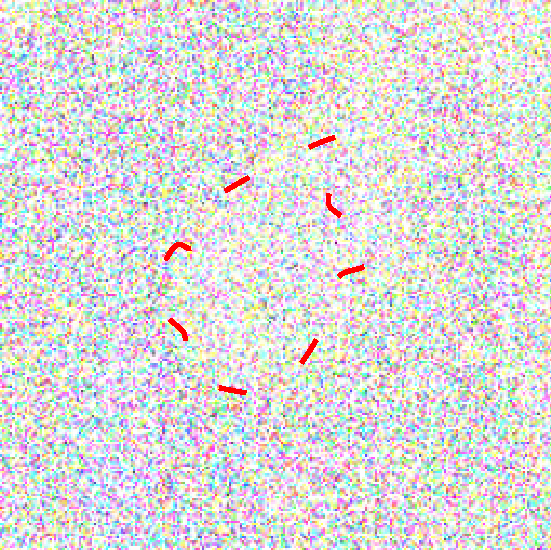
\includegraphics[width=\linewidth]{graphics/ResNet-50/LesionOutline.pdf}
            \caption{Shape of skin lesion found in adversarial ``noise''\\}
            \label{LesionShape}
          \end{subfigure}
          \begin{subfigure}{.4\linewidth}
            \centering
            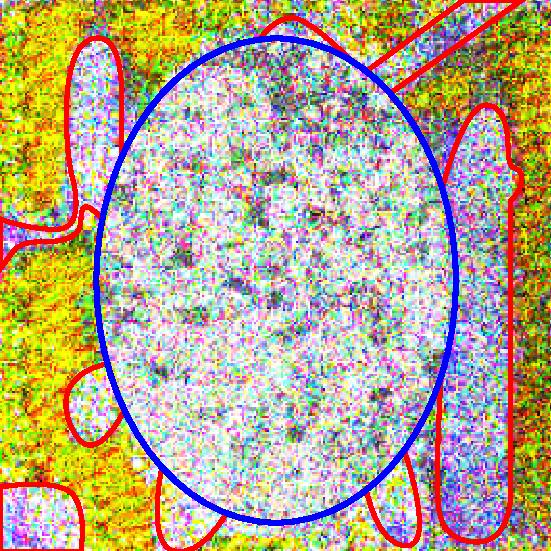
\includegraphics[width=\linewidth]{graphics/ResNet-50/EyeShapeDivergence.pdf}
            \caption{Divergence from shape of eye\\}
            \label{EyeShapeDivergence}
          \end{subfigure}
          \caption{Shape information carried over into perturbations}
        \end{figure}

        \begin{figure}[h]
          \centering
          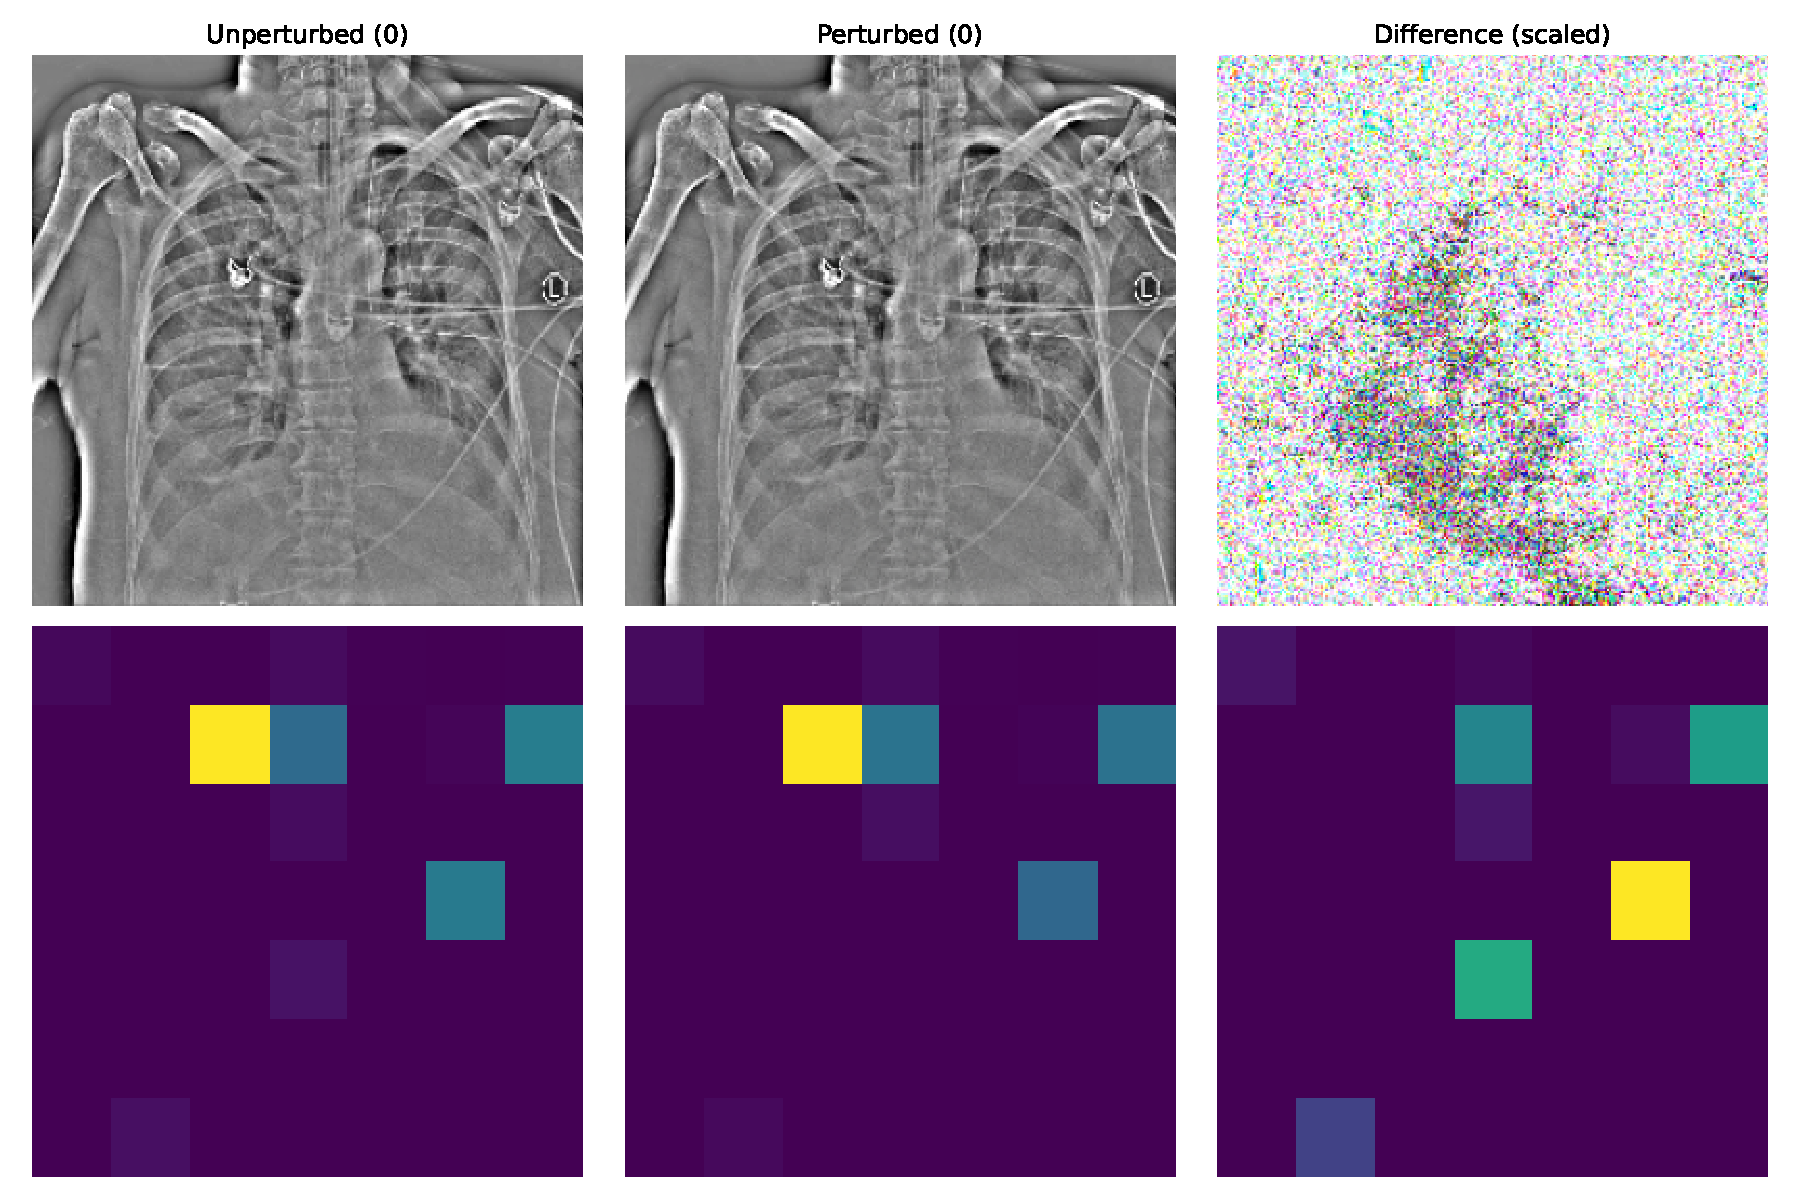
\includegraphics[width=\linewidth]{graphics/ResNet-50/pneumo_with_attention.pdf}
          \caption{Comparison of activation maps (with attention) for perturbed and unperturbed chest x-ray}
          \label{PneumoWithAttention}
        \end{figure}

        \begin{figure}[h]
          \centering
          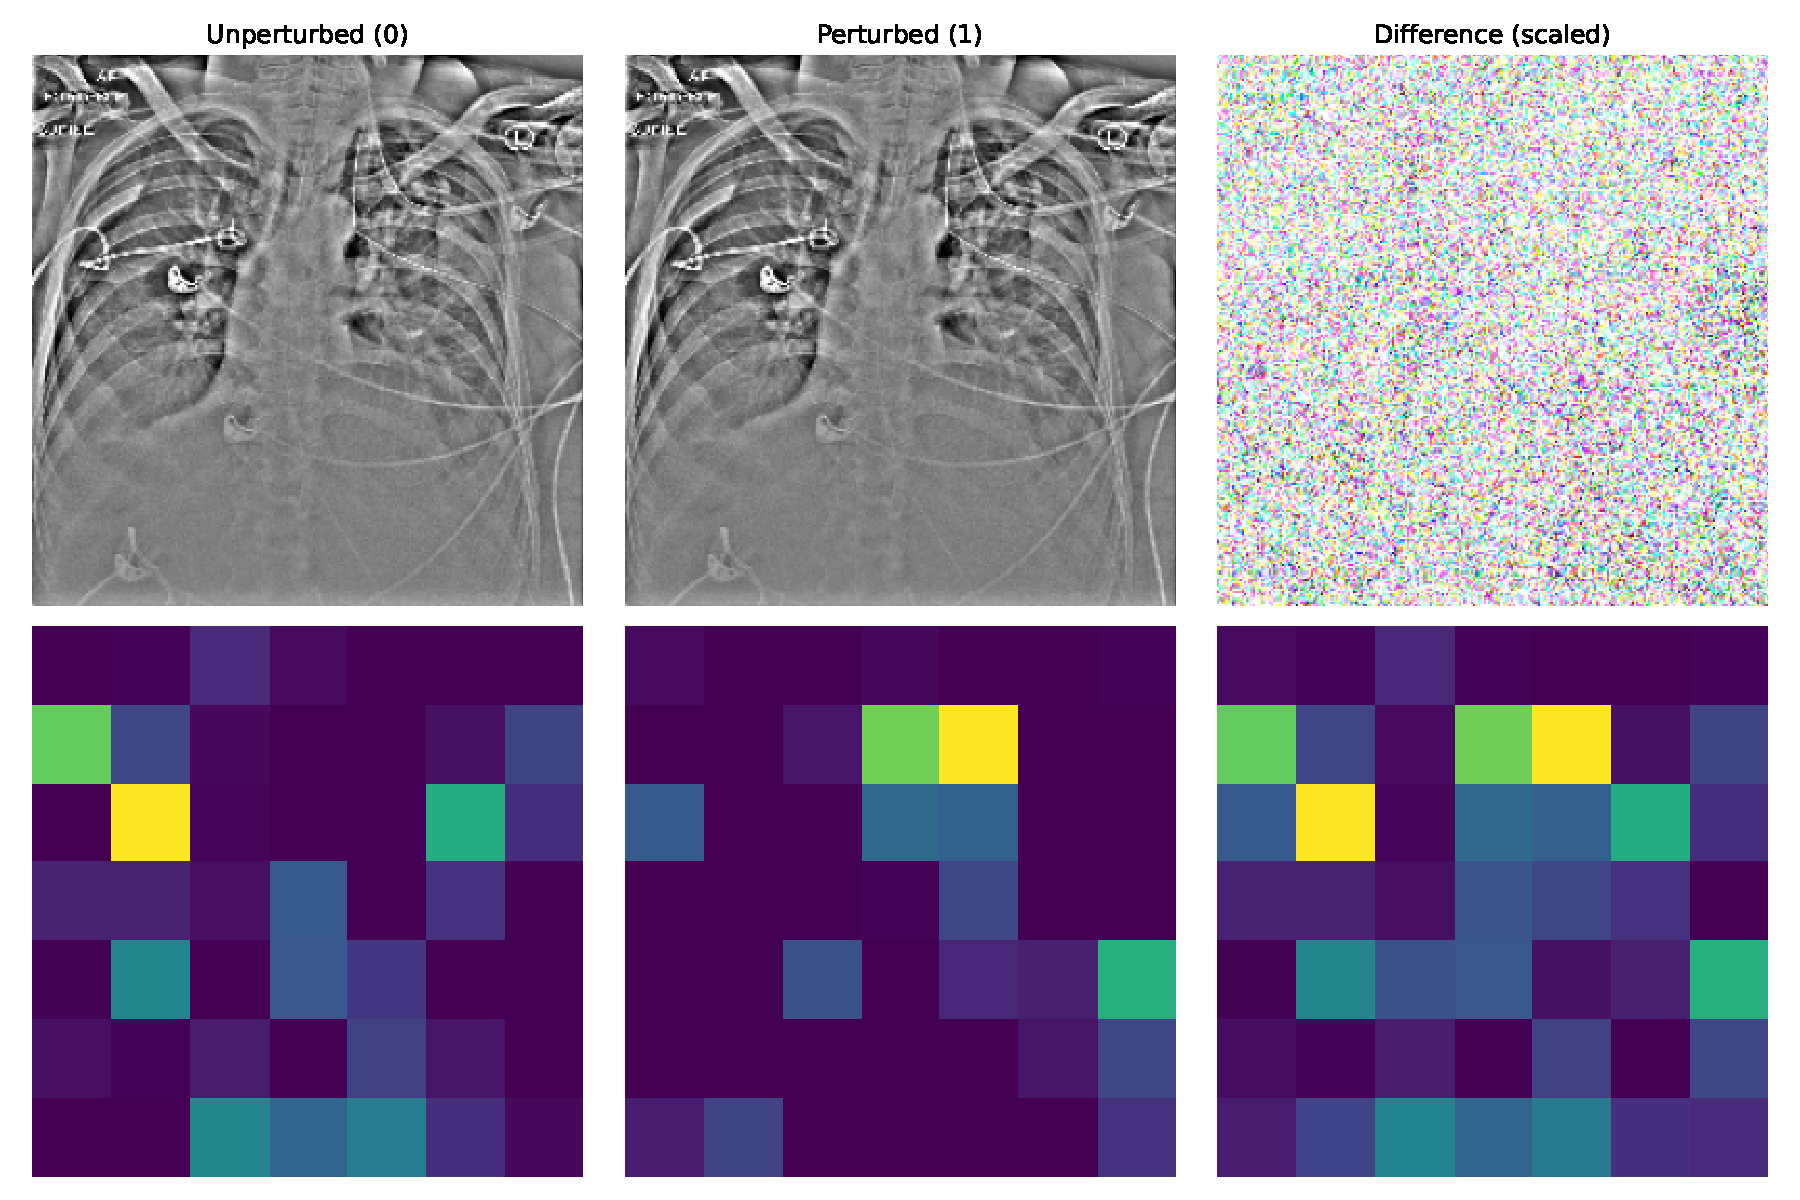
\includegraphics[width=\linewidth]{graphics/ResNet-50/different_maps.pdf}
          \caption{Comparison of activation maps (without attention) for perturbed and unperturbed chest x-ray}
          \label{DifferentMaps}
        \end{figure}

        In the attacks tailored to the fundoscopic image models, perturbations introduced dark splotchy patterns to the eye area (Fig. \ref{CottonWool}). Based on diagnostic literature, these spots could be ``attempts'' by the attack to emulate cotton-wool spots or hemorrhages, key indicators of diabetic retinopathy \cite{WillsEye}. Similar patterns appear in the perturbations for the chest x-ray model with attention (Fig. \ref{PneumoWithAttention}) (these spots are larger and less speckled), though these do not appear similar to the key indicators of pneumothoraces (air in pleural space, misplaced lung edge, less distinct lung markings, etc.) \cite{UnofficialGuide}, it remains unclear whether the attack could be emulating these features indirectly.

        \begin{figure}[h]
          \centering
          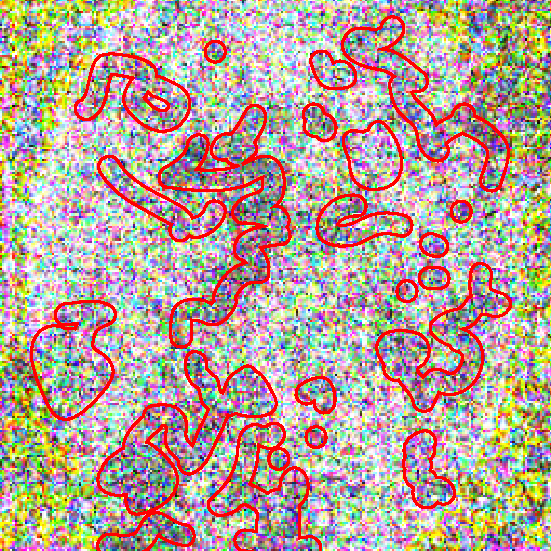
\includegraphics[width=0.5\linewidth]{graphics/ResNet-50/cotton_wool.pdf}
          \caption{Dark splotches in perturbation of fundoscopic images}
          \label{CottonWool}
        \end{figure}

        While the activation maps for the dermatoscopic and fundoscopic image models were invariant to perturbation, the chest x-ray model without attention occasionally produced very different activation maps under adversarial attacks (Fig. \ref{DifferentMaps}). However, this was only true under successful attacks (of which there were few).

        For all three datasets, models with attention produced activation maps that were very different from their baseline counterparts; in most cases, the regions of highest activation did not match across models. Additionally, the activation maps for the chest x-ray model with attention were highly focused, typically having a single region of significance (Fig. \ref{DifferentMaps}).

        

      \subsubsection{InceptionResNetV2 Models}
      
    \subsection{Conclusion} % Result, contribution, future work
      
    
%%%%%%%%% REFERENCES
{\small
\bibliographystyle{ieee_fullname}
\bibliography{egbib}
}

\pagebreak
\appendix

\end{document}
